% article example for classicthesis.sty
\documentclass[10pt,a4paper]{article} % KOMA-Script article scrartcl
\usepackage{lipsum}     %lorem ipsum text
\usepackage{titlesec}   %Section settings
\usepackage{titling}    %Title settings
\usepackage[margin=10em]{geometry}  %Adjusting margins
\usepackage{setspace}
\usepackage{listings}
\usepackage{amsmath}    %Display equations options
\usepackage{amssymb}    %More symbols
\usepackage{xcolor}     %Color settings
\usepackage{pagecolor}
\usepackage{mdframed}
\usepackage[spanish]{babel}
\usepackage[utf8]{inputenc}
\usepackage{longtable}
\usepackage{multicol}
\usepackage{graphicx}
\graphicspath{ {./Images/} }
\setlength{\columnsep}{1cm}

% ====| color de la pagina y del fondo |==== %
\pagecolor{black}
\color{white}



\begin{document}
    %========================{TITLE}====================%
    \title{\rmfamily\normalfont\spacedallcaps{ Nociones Basicas Teoria de Grafos }}
    \author{\spacedlowsmallcaps{Rodrigo Castillo}}
    \date{\today} 
    
    \maketitle
     

     % ====| Loguito |==== %
    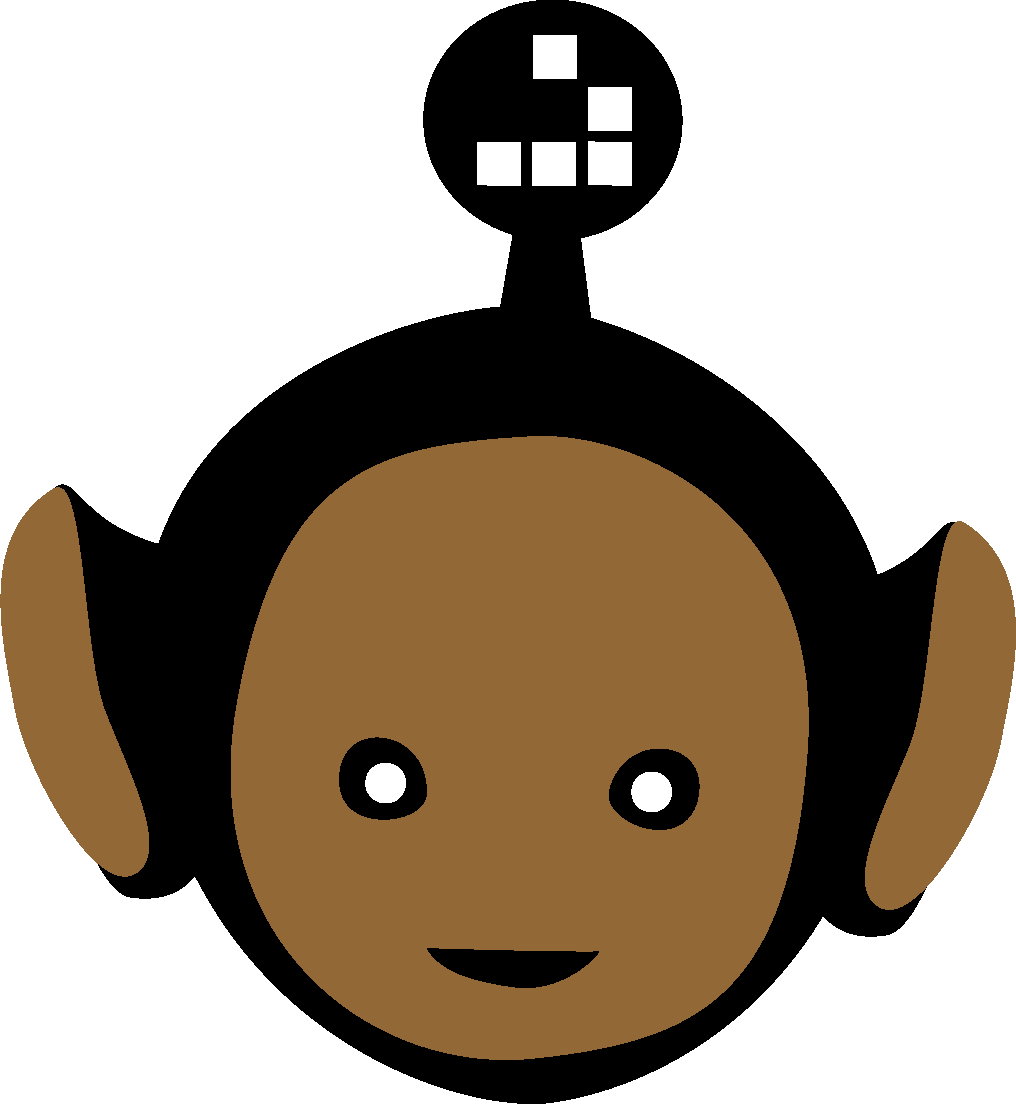
\includegraphics[width=0.1\linewidth]{negro_cara.png}
    %=======================NOTES GOES HERE===================%
    \section{Problema de los puentes de konigsberg}
        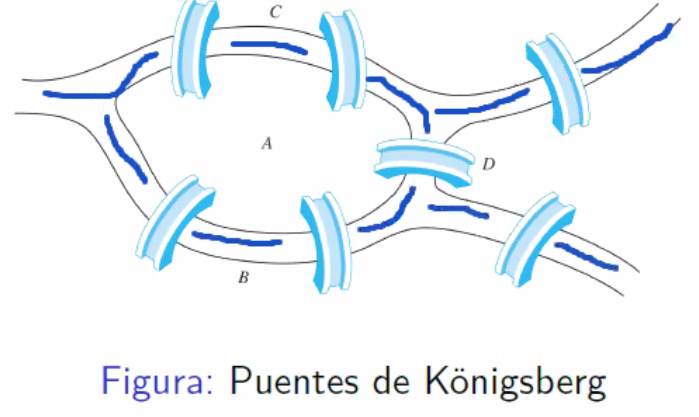
\includegraphics[width=0.8\linewidth]{puentes.png} 
        \\con la teoría de grafos se demuestra que es imposible recorrer todas
        las islas pasando unicamente solo una vez por cada puente  
        \\ yo ya sé que la crema de la demostración es porque hay un número
        impar de puentes pero me tengo que quedar callado porque pues nadie
        sabe nada piu piu piu piu gqq 
    \section{Definicion de grafo:}
        un grafo $ G  $  es una terna que consiste en un conjunto
        de vertices $ V(G)  $  , un conjunto de atistas $ E(G)  $
        y una relacion que asocia cada arista con un par de
        vertices 
        \\ existe una relacion que asocia a cada arista con un par de vértices 
        \\ para el problema de los puentes tenemos que:

        \\ $ V(G)  $   = $ {A,B,C,D}  $  
        \\ $ E(G)  $  = $ e_1 , e_2 , e_3 , ... , e_7  $  
     \section{relacion de adyacencia}
         dos vertices u y v son adyacentes si $ u $ y $ v  $  son extremos de
         una arista $ e   $ (trivial) 
     \section{blucle o lazo}
         un bucle o lazo  es una arista cuyos extremos son iguales
     \section{aristas multiples o paralelas}
         dos o mas aristas son multiples o paralelas si tienen el mismo par de extremos
      \section{grafo simple}
          un grafo simple $ G = (V,E)  $  es un grafo sin bucles
          ni aristas multiples donde $ E  $  es un conjunto de
          pares no orientados de vértices
          
          \\ $ V = {a,b,c,d}  $  
          \\ $ E = {ab,bc,cd,da}  $  
          \\esto solo se puede usar cuando no hay aristas multiples
      \section{grafo finito}
          un grafo es vinito si $ V(G)  $  y $ E(G)  $  son conjuntos finitos 
      \section{grafo nulo}
          un grafo es nulo si $ V(G)  $  y $ E(G)  $   = Null
      \section{grafo complementario}
          el complemento $ G  $  de un grafo simple $ Q  $  es el grafo simple
          con el conjuto de vertices $ V(G)  $  definido por $ uv   $
          pertenece a $ Q(G)  $  sii $ uv  $  no pertenece a $ E(G)  $  
            







    %=======================NOTES ENDS HERE===================%
    
    % bib stuff
    \nocite{*}
    \addtocontents{toc}{\protect\vspace{\beforebibskip}}
    \addcontentsline{toc}{section}{\refname}    
    \bibliographystyle{plain}
    \bibliography{../Bibliography}
\end{document}
